\documentclass[nobib]{tufte-handout}

%\\geometry{showframe}% for debugging purposes -- displays the margins

\newcommand{\bra}[1]{\left(#1\right)}
\usepackage{clrscode3e}
\usepackage{hyperref}
\usepackage[activate={true,nocompatibility},final,tracking=true,kerning=true,spacing=true,factor=1100,stretch=10,shrink=10]{microtype}
\usepackage{color}

% Fixes captions and images being cut off
\usepackage{marginfix}

\usepackage{circuitikz}
\usepackage{amsmath,amsthm}
\usetikzlibrary{shapes}
\usetikzlibrary{positioning}
\usetikzlibrary{arrows}

% Set up the images/graphics package
\usepackage{graphicx}
\setkeys{Gin}{width=\linewidth,totalheight=\textheight,keepaspectratio}
\graphicspath{{.}}

\title{Notes for ECE 20001 - EE Fundementals I}
\author[Ezekiel Ulrich]{Ezekiel Ulrich}
\date{\today}  % if the \date{} command is left out, the current date will be used

% The following package makes prettier tables.  We're all about the bling!
\usepackage{booktabs}

% The units package provides nice, non-stacked fractions and better spacing
% for units.
\usepackage{units}

% The fancyvrb package lets us customize the formatting of verbatim
% environments.  We use a slightly smaller font.
\usepackage{fancyvrb}
\fvset{fontsize=\normalsize}

% Small sections of multiple columns
\usepackage{multicol}

% These commands are used to pretty-print LaTeX commands
\newcommand{\doccmd}[1]{\texttt{\textbackslash#1}}% command name -- adds backslash automatically
\newcommand{\docopt}[1]{\ensuremath{\langle}\textrm{\textit{#1}}\ensuremath{\rangle}}% optional command argument
\newcommand{\docarg}[1]{\textrm{\textit{#1}}}% (required) command argument
\newenvironment{docspec}{\begin{quote}\noindent}{\end{quote}}% command specification environment
\newcommand{\docenv}[1]{\textsf{#1}}% environment name
\newcommand{\docpkg}[1]{\texttt{#1}}% package name
\newcommand{\doccls}[1]{\texttt{#1}}% document class name
\newcommand{\docclsopt}[1]{\texttt{#1}}% document class option name

% Define a custom command for definitions
\newcommand{\defn}[2]{\noindent\textbf{#1}:\ #2}

\begin{document}

\maketitle

\begin{abstract}
These are lecture notes for fall 2023 ECE 20001 at Purdue. Modify, use, and distribute as you please.
\end{abstract}

\tableofcontents

\section{Course Introduction}

This course covers fundamental concepts and applications 
for electrical and computer engineers as well as for engineers
 who need to gain a broad understanding of these disciplines. 
 The course starts by the basic concepts of charge, current, 
 and voltage as well as their expressions with regards to 
 resistors and resistive circuits. Essential concepts, 
 devices, theorems, and applications of direct-current (DC), 
 1st order, and alternating-current (AC) circuits are 
 subsequently discussed. Besides electrical devices and 
 circuits, basic electronic components including diodes and 
 transistors as well as their primary applications are also 
 discussed. For more information, see the syllabus. 

\section{Equations}

\begin{enumerate}
    \item $P = \frac{dW}{dt} = IV$
    \item $I = \frac{dq}{dt}$
    \item $V = \frac{W}{q}$
    \item $R = \frac{\rho L}{A}$
    \item Ohm's Law: $V=IR$
    \item Coulomb's Law: $\vec{F} = \frac{1}{4\pi \epsilon_0}\frac{q_1 q_2}{r^2}\hat{r}$
    \item Kirchhoff's Voltage Law: 
    \item Conductance: $G = \frac{1}{R}$
\end{enumerate}

\pagebreak

\section{Charge, current, voltage, and power}
Before we begin a discussion
of electrical engineering, we will want an
understanding of some important concepts. 

\defn{Charge}{A fundemental property of matter.} Charge
is measured in units of Coulombs (C) and 
arises from aggregates of charged 
fundemental particles like electrons.

\defn{Current}{The rate of flow of charge.} Typically,
we think of current as occuring in a circuit, a loop
through which charge can flow. Current can
be mathematically defined as $I = \frac{dq(t)}{dt}$, where 
$q(t)$ is the charge at time $t$. Current therefore has units
of Coulombs per second (C/s). 

\defn{Voltage}{The difference in electric potential energy
between two points, per unit charge.} Voltage thus has units of
$\frac{J}{C}$. or Volts (V).
Intuitively, a stronger voltage source (such
as a battery) will result in a higher current on 
identical wires. Imagine a voltage source
as a concentration of negative charges on
one side and positive charges on the other. 
If we hook both ends up to a conducting wire and place 
an electron in the wire, it will be repelled 
from the negative side and attracted to the
positive side. The electron has a high
potential energy near the concentration of
negative charge, and a low potential energy
near the positive charges. The difference
between these potentials is the voltage. This should
make it clear that voltage must always be
defined as across two points, each with its
electric potential. A good note is that
voltage can be negative (if the electric 
potential at the second point measured is higher)
and it may not be constant with time. 

\defn{Power}{The rate of doing work, or changing energy.} 
Mathematically, $P = \frac{dW}{dt} = IV$ and has units of Watts (W).
In a closed system, power is always balanced: whatever 
is put out by sources is consumed by
loads. Thus, in a closed circuit, $\sum P = 0$ This
is an important point, so allow me to illustrate it with 
an example. Say we have the below circuit:

\begin{circuitikz} \draw
    (0,-2) -- (0,2)
      (0,2) -- (3,2)
      (3, 2) -- (3, 0)
      (0, -2) -- (9, -2)
      (0, 0) -- (9,0)
      (3, -2) -- (3, 0)
      (6, -2) -- (6, 0)
      (9, -2) -- (9, 0)
    ;
    \node[draw, rectangle, minimum width=0.5cm, minimum height=0.5cm] at (1.5,2) {G}
    (1.5,2.25) node[above] {$+ 4 V -$}

    (1.5,2) to [short,i=$1A$] (0,2);

    \node[draw, rectangle, minimum width=0.5cm, minimum height=0.5cm] at (1.5,0) {B}
    (1.5,0.25) node[above] {$+ 4 V -$}

    (0,0) to [short,i=$4A$] (1.5,0);

    \node[draw, rectangle, minimum width=0.5cm, minimum height=0.5cm] at (0,-1) {A}
    (-.25,-1) node[label={[rotate=90]above:$- 10V +$}] {};

    \draw (0,-.25) to[short, i=$3A$] (0, 0);

    \node[draw, rectangle, minimum width=0.5cm, minimum height=0.5cm] at (3,-1) {C}
    (2.75,-1) node[label={[rotate=90]above:$- 6V +$}] {};

    \draw (3,0) to[short, i=$5A$] (3, -.25);

    \node[draw, rectangle, minimum width=0.5cm, minimum height=0.5cm] at (6,-1) {E}
    (5.75,-1) node[label={[rotate=90]above:$+ 2V -$}] {};

    \draw (6,0) to[short, i=$-1A$] (6, -.25);

    \node[draw, rectangle, minimum width=0.5cm, minimum height=0.5cm] at (4.5,0) {D}
    (4.5,.25) node[above] {$+ 8V -$};

    \draw (3,0) to[short, i=$-2A$] (4.5, 0);

    \node[draw, rectangle, minimum width=0.5cm, minimum height=0.5cm] at (9,-1) {F}
    (8.75,-1) node[label={[rotate=90]above:$- 2V +$}] {};

    \draw (9,-1) to[short, i=$I$] (9, 0);

\end{circuitikz}

We know $\sum P_i = \sum V_i I_i = 0$. Let's keep track 
of each $P_i$ in a table, not forgetting passive
sign convention:
\begin{table}[ht]
    \centering
    \begin{tabular}{|c c|}
    \hline
    Symbol & Watts \\
    \hline
    $P_A$ & -30 \\
    $P_B$ & 16 \\ 
    $P_C$ & 30 \\
    $P_D$ & -16 \\
    $P_E$ & 2 \\
    $P_F$ & -2$I$ \\
    $P_G$ & -4 \\
    \hline
    \end{tabular}
    \caption{Power absorbed}
    \label{tab:powerabsorbtable}
\end{table}
Summing the rows of this table, we have 
$\sum P_i = 2I - 2 = 0$, implying $I = 1$.

In the previous example, we had current flowing
both into and out of the positive terminals
of elements. We also had negative currents. Let's define 
how to handle signage in circuits:

\defn{Passive sign convention}{Defines current as going into 
positive voltage node of a component.} The component
is labeled a \emph{load} or a \emph{passive device}.
We call it this because the component
consumes power. If a current is negative,
it is flowing in the opposite direction shown by the
arrow.
\begin{marginfigure}
    \centering
    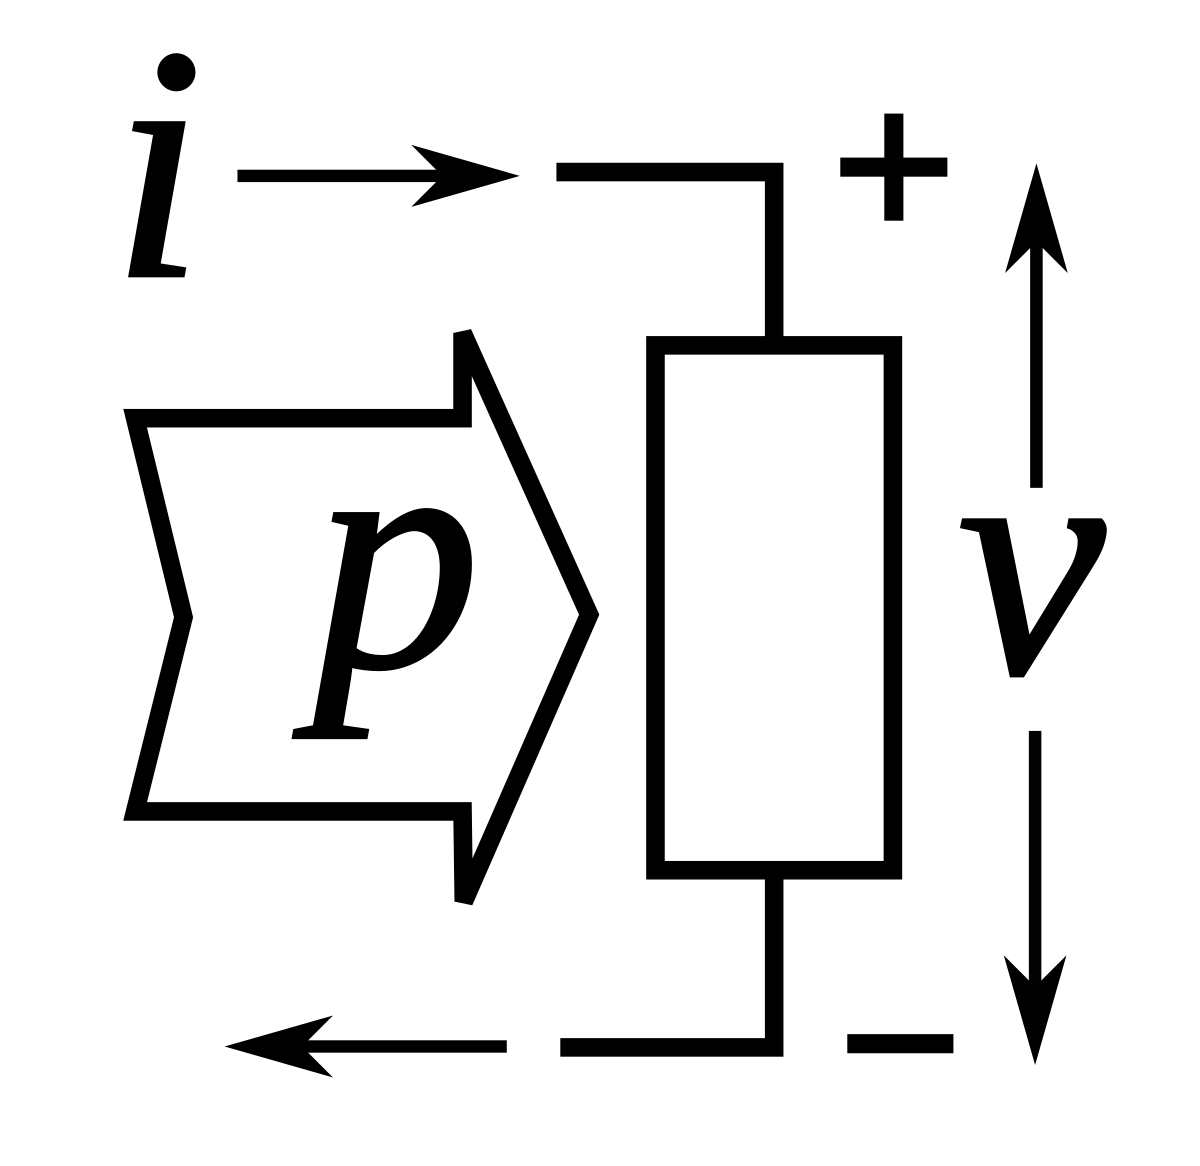
\includegraphics{images/Passive_sign_convention.svg.png}
    \caption{Passive sign convention}
    \label{fig:psc} 
\end{marginfigure}
It's useful to have an idea of the components of circuit
schematics (visual representations of a circuit). Below is a list 
of the terms that will be used in this course:
\begin{itemize}
    \item Elements: The term elements means "components and sources."
    \item Symbols: Elements are represented in schematics by symbols. 
    Symbols for common 2-terminal elements are displayed to the right.
    
\begin{marginfigure}
    \centering
    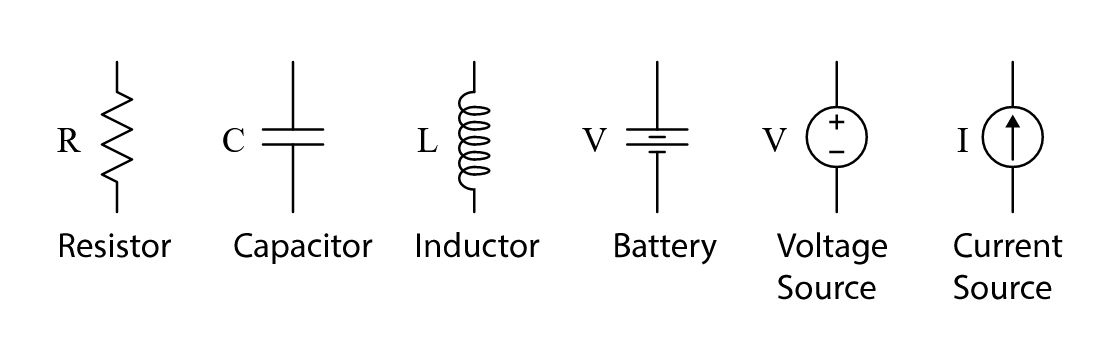
\includegraphics{images/symbols.png}
    \caption{Common circuit symbols}
    \label{fig:symbols}
\end{marginfigure} 

    \item Lines: Connections between elements are drawn as lines, 
    which we often think of as "wires". On a schematic, 
    these lines represent perfect conductors with zero resistance. 
    Every component or source terminal touched by a line is at the same voltage.
    \item Dots: Connections between lines can be indicated by dots. 
    Dots are an unambiguous indication that lines are connected. 
    If the connection is obvious, you don't have to use a dot.
\end{itemize}
Check out the circuit schematic below and see how many components you 
can identify!
\begin{center}
    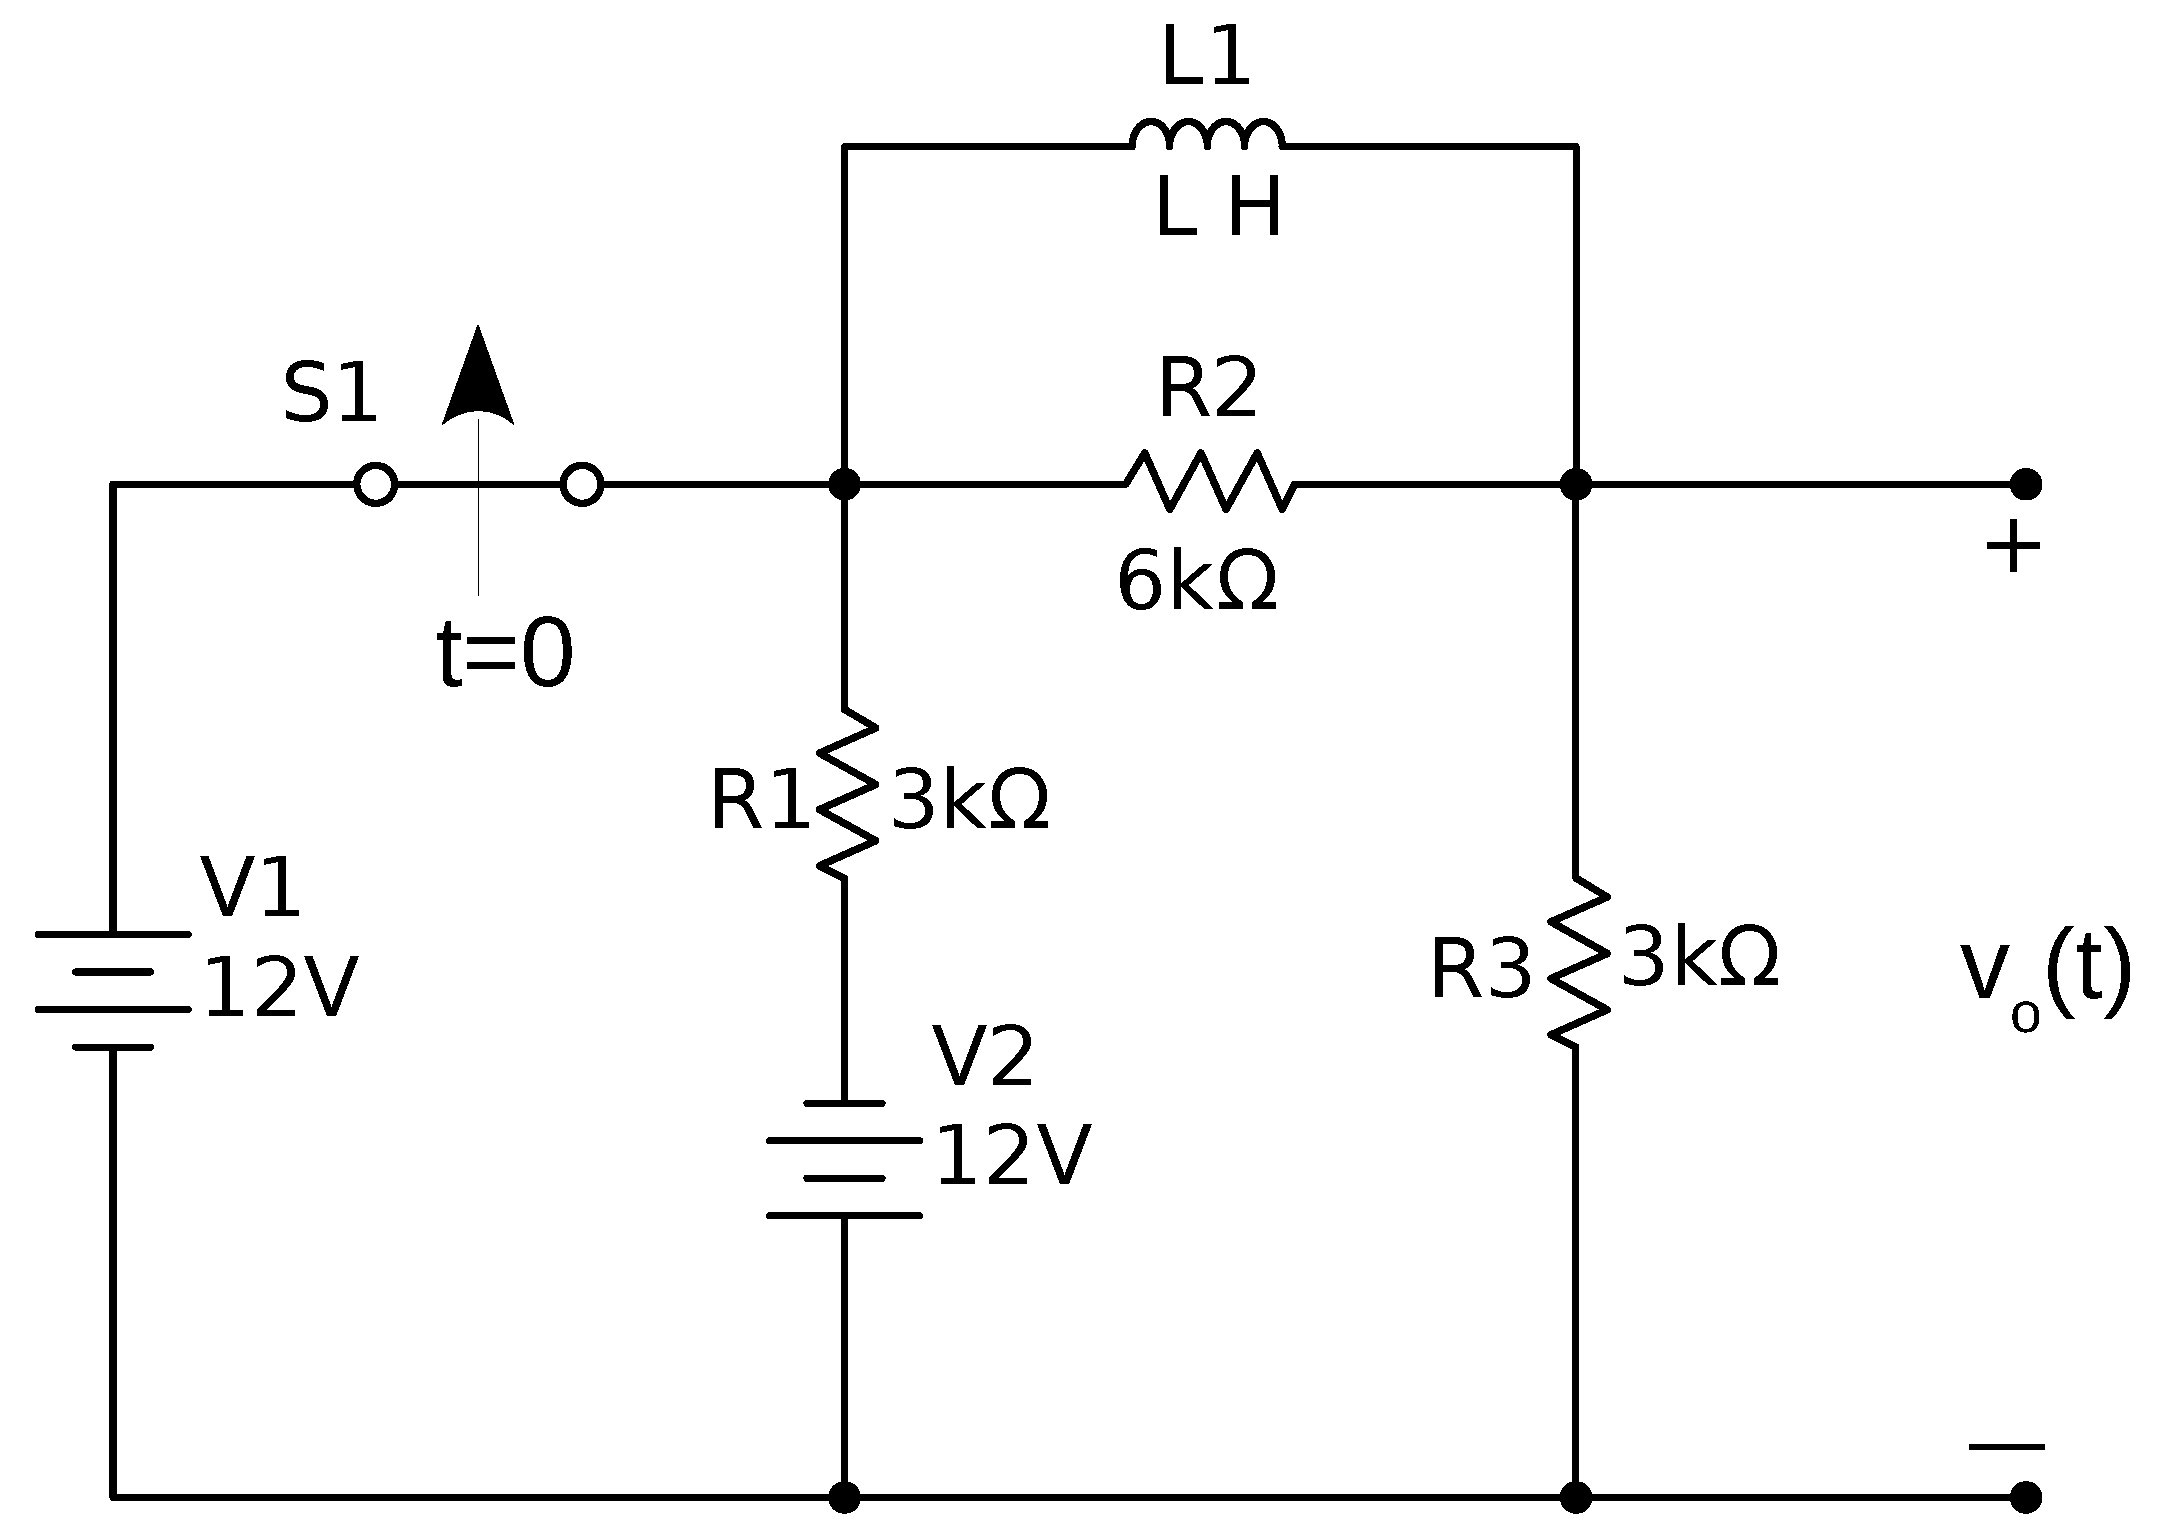
\includegraphics[width=\textwidth/2]{images/PS0_CapacitorCircuit.png}
\end{center}

\section{(In)dependent sources, connections, resistance and Ohm's Law}
Now, on to what circuits are doing. For interesting things
to happen we need electrons flowing through those wires,
and for that we need sources. There are two types: independent and dependent.
Independent sources are voltage sources or current sources 
that maintain a constant value regardless of the rest of the 
circuit. They are not influenced by the circuit's current or 
voltage conditions. There are two main types of independent 
sources:
\begin{itemize}
    \item \defn{Independent voltage source}{Maintains a constant 
    voltage across its terminals, regardless of the current 
    flowing through it. It is typically represented by a 
    symbol with a plus sign and a minus sign, indicating 
    the polarity of the voltage.} A battery maintaining a constant
    voltage of 9 V is an example of an independent voltage source.
    \begin{marginfigure}
        \centering
        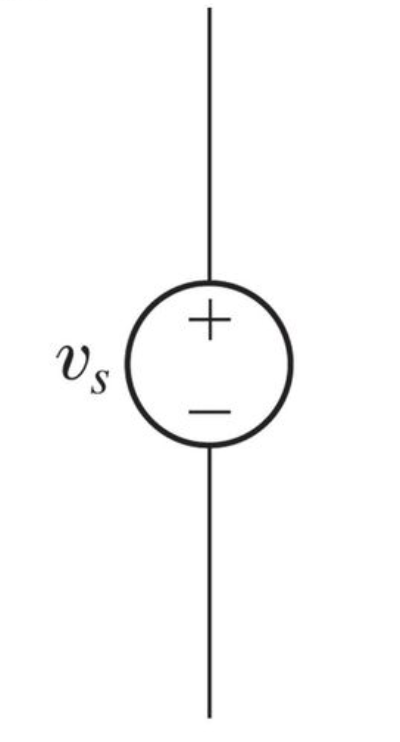
\includegraphics{images/independentvoltagesource.png}
        \caption{inependent voltage source}
        \label{fig:independentvoltagesource}
    \end{marginfigure} 

    \item \defn{Independent current source}{Maintains a constant 
    current through its terminals, regardless of the 
    voltage across it. It is usually represented by 
    a symbol with an arrow indicating the 
    direction of current flow.} Consider a current source that 
    provides a constant current of 2 amperes. This source 
    will deliver a current of 2A through any component 
    connected to it, regardless of the 
    voltage across the component.
    \begin{marginfigure}
        \centering
        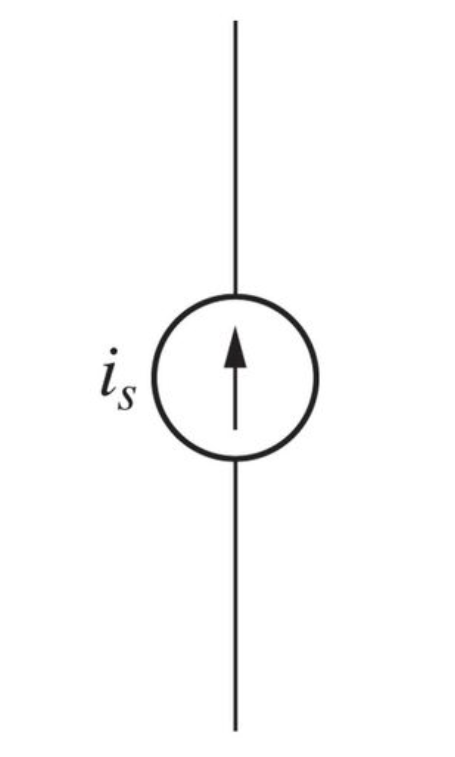
\includegraphics{images/independentcurrentsource.png}
        \caption{Independent current source}
        \label{fig:independentcurrentsource}
    \end{marginfigure} 
    
\end{itemize}
Contrasted with independent sources are 
dependent sources. Dependent sources are sources 
whose values are 
dependent on other variables within the circuit. 
These sources are used to model components whose 
behavior changes according to the conditions in 
the circuit. There are four types of dependent sources:
\begin{itemize}
    \item \defn{Voltage-Controlled Voltage Source (VCVS)}{
    This type of dependent source generates a voltage 
    that is proportional to the voltage across a 
    separate part of the circuit.}
    \begin{marginfigure}
        \centering
        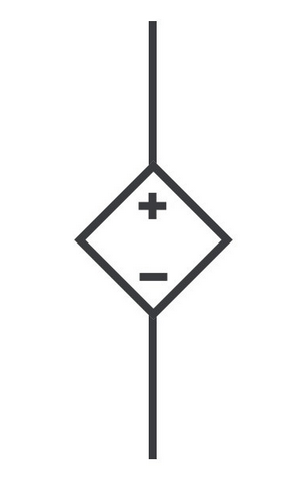
\includegraphics{images/dependentvoltagesource.png}
        \caption{Dependent voltage source}
        \label{fig:dependentvoltagesource}
    \end{marginfigure} 

    \item \defn{Current-Controlled Current Source (CCCS)}{
    This type of dependent source generates a current 
    that is proportional to the current flowing 
    through a different part of the circuit.}
    \begin{marginfigure}
        \centering
        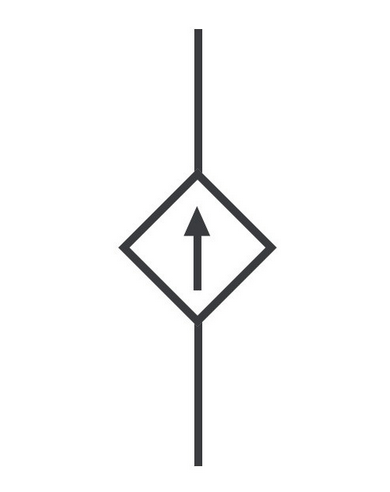
\includegraphics{images/dependentcurrentsource.png}
        \caption{Dependent current source}
        \label{fig:dependentcurrentsource}
    \end{marginfigure} 


    \item \defn{Voltage-Controlled Current Source (VCCS)}{
    This type of dependent source generates a 
    current that is proportional to the 
    voltage across a different part of the 
    circuit.}
    \item \defn{Current-Controlled Voltage Source (CCVS)}{
    This type of dependent source generates a 
    voltage that is proportional to the 
    current flowing through a separate part 
    of the circuit.}
\end{itemize}
In both the independent and dependent case, we assume
the sources are ideal. There are two
critical attributes of ideal sources. First, their value remains unchanged indefi-
nitely. Second, they can deliver any amount of power needed by their loads.

Now that we have a good idea of circuit components, we can look 
at important configurations. These are the most useful:

\defn{Series Combination}{In a series combination, the elements 
are connected with end to end in contact, such that 
current flow is equal in all the elements in the 
combination}

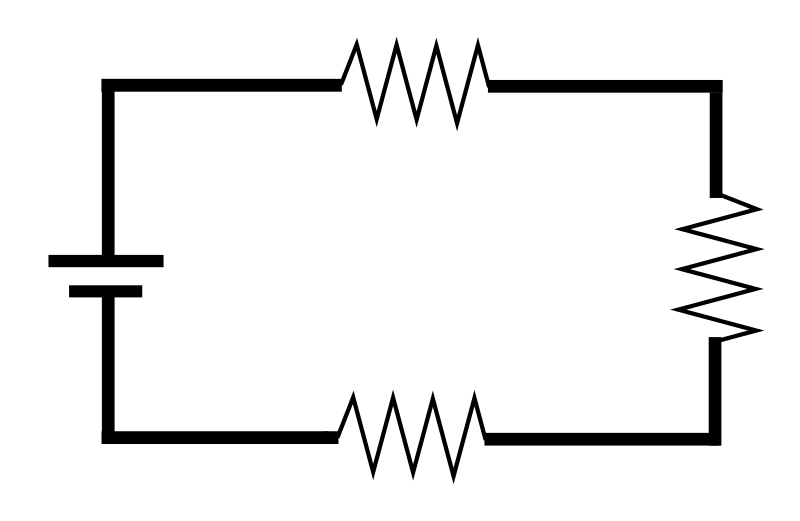
\includegraphics[width=\textwidth/2]{images/Series_circuit.svg.png}

\defn{Parallel Combination}{When two or more resistances are 
connected between the same two points, they are said to be 
connected in parallel combination. In this case voltage is equal
across all elements}

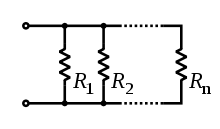
\includegraphics[width=\textwidth/2]{images/220px-Resistors_in_parallel.svg.png}

Turning off a voltage source is equivalent to replacing it with a 
short circuit (line). Turning off a current source is equivalent to replacing it with an
open circuit (broken line). Also equivalent to an open
circuit is a resistor with infinite resistance. 
Resistance is a measure of how hard it is to shove current
through a resistor. The harder it is, the higher the
resistance. It's given by $R = \frac{\rho L}{A} = \frac{V}{I}$, where $\rho$ 
is the resistivity, $L$ is the length of the resistor, and $A$ is the 
cross-sectional area of the resistor. The reciprocal of
resistance is conductance ($G = \frac{1}{R}$). We can relate 
voltage, current and resistance with \emph{Ohm's Law}.

\defn{Ohm's Law}{$V = IR$.} This law is fundemental to EE and will
occur repeatedly throughout the course. 

\section{Kirchhoff's Laws, resistor combinations, and voltage/current division}


\end{document}
